%package list
\documentclass{article}
\usepackage[top=3cm, bottom=3cm, outer=3cm, inner=3cm]{geometry}
\usepackage{multicol}
\usepackage{graphicx}
\usepackage{url}
%\usepackage{cite}
\usepackage{hyperref}
\usepackage{array}
%\usepackage{multicol}
\newcolumntype{x}[1]{>{\centering\arraybackslash\hspace{0pt}}p{#1}}
\usepackage{natbib}
\usepackage{pdfpages}
\usepackage{multirow}
\usepackage[normalem]{ulem}
\useunder{\uline}{\ul}{}
\usepackage{svg}
\usepackage{xcolor}
\usepackage{listings}
\lstdefinestyle{ascii-tree}{
    literate={├}{|}1 {─}{--}1 {└}{+}1 
  }
\lstset{basicstyle=\ttfamily,
  showstringspaces=false,
  commentstyle=\color{red},
  keywordstyle=\color{blue}
}
%\usepackage{booktabs}
\usepackage{caption}
\usepackage{subcaption}
\usepackage{float}
\usepackage{array}

\newcolumntype{M}[1]{>{\centering\arraybackslash}m{#1}}
\newcolumntype{N}{@{}m{0pt}@{}}


%%%%%%%%%%%%%%%%%%%%%%%%%%%%%%%%%%%%%%%%%%%%%%%%%%%%%%%%%%%%%%%%%%%%%%%%%%%%
%%%%%%%%%%%%%%%%%%%%%%%%%%%%%%%%%%%%%%%%%%%%%%%%%%%%%%%%%%%%%%%%%%%%%%%%%%%%
\newcommand{\itemEmail}{rvaldiviase@unsa.edu.pe}
\newcommand{\itemStudent}{Ryan Fabian Valdivia Segovia}
\newcommand{\itemCourse}{Fundamentos de la programación 2}
\newcommand{\itemCourseCode}{1701213}
\newcommand{\itemSemester}{II}
\newcommand{\itemUniversity}{Universidad Nacional de San Agustín de Arequipa}
\newcommand{\itemFaculty}{Facultad de Ingeniería de Producción y Servicios}
\newcommand{\itemDepartment}{Departamento Académico de Ingeniería de Sistemas e Informática}
\newcommand{\itemSchool}{Escuela Profesional de Ingeniería de Sistemas}
\newcommand{\itemAcademic}{2023 - B}
\newcommand{\itemInput}{Del 06 de Diciembre 2023}
\newcommand{\itemOutput}{Al 11 de Diciembre 2023}
\newcommand{\itemPracticeNumber}{12}
\newcommand{\itemTheme}{Clase Soldado - Menú}
%%%%%%%%%%%%%%%%%%%%%%%%%%%%%%%%%%%%%%%%%%%%%%%%%%%%%%%%%%%%%%%%%%%%%%%%%%%%
%%%%%%%%%%%%%%%%%%%%%%%%%%%%%%%%%%%%%%%%%%%%%%%%%%%%%%%%%%%%%%%%%%%%%%%%%%%%

\usepackage[english,spanish]{babel}
\usepackage[utf8]{inputenc}
\AtBeginDocument{\selectlanguage{spanish}}
\renewcommand{\figurename}{Figura}
\renewcommand{\refname}{Referencias}
\renewcommand{\tablename}{Tabla} %esto no funciona cuando se usa babel
\AtBeginDocument{%
	\renewcommand\tablename{Tabla}
}

\usepackage{fancyhdr}
\pagestyle{fancy}
\fancyhf{}
\setlength{\headheight}{30pt}
\renewcommand{\headrulewidth}{1pt}
\renewcommand{\footrulewidth}{1pt}
\fancyhead[L]{\raisebox{-0.2\height}{
\includegraphics[width=3cm]{img/logo_episunsa.png}}}
\fancyhead[C]{\fontsize{7}{7}\selectfont	\itemUniversity \\ \itemFaculty \\ \itemDepartment \\ \itemSchool \\ \textbf{\itemCourse}}
\fancyhead[R]{\raisebox{-0.2\height}{
\includegraphics[width=1.2cm]{img/logo_abet}}}
\fancyfoot[L]{Estudiante Ryan Valdivia}
\fancyfoot[C]{\itemCourse}
\fancyfoot[R]{Página \thepage}

% para el codigo fuente
\usepackage{listings}
\usepackage{color, colortbl}
\definecolor{dkgreen}{rgb}{0,0.6,0}
\definecolor{gray}{rgb}{0.5,0.5,0.5}
\definecolor{mauve}{rgb}{0.58,0,0.82}
\definecolor{codebackground}{rgb}{0.95, 0.95, 0.92}
\definecolor{tablebackground}{rgb}{0.8, 0, 0}

\lstset{frame=tb,
	language=bash,
	aboveskip=3mm,
	belowskip=3mm,
	showstringspaces=false,
	columns=flexible,
	basicstyle={\small\ttfamily},
	numbers=none,
	numberstyle=\tiny\color{gray},
	keywordstyle=\color{blue},
	commentstyle=\color{dkgreen},
	stringstyle=\color{mauve},
	breaklines=true,
	breakatwhitespace=true,
	tabsize=3,
	backgroundcolor= \color{codebackground},
}

\begin{document}
	
	\vspace*{10px}
	
	\begin{center}	
		\fontsize{17}{17} \textbf{ Informe de Laboratorio \itemPracticeNumber}
	\end{center}
	\centerline{\textbf{\Large Tema: \itemTheme}}
	%\vspace*{0.5cm}	

	\begin{flushright}
		\begin{tabular}{|M{2.5cm}|N|}
			\hline 
			\rowcolor{tablebackground}
			\color{white} \textbf{Nota}  \\
			\hline 
			     \\[30pt]
			\hline 			
		\end{tabular}
	\end{flushright}	

	\begin{table}[H]
		\begin{tabular}{|x{4.7cm}|x{4.8cm}|x{4.8cm}|}
			\hline 
			\rowcolor{tablebackground}
			\color{white} \textbf{Estudiante} & \color{white}\textbf{Escuela}  & \color{white}\textbf{Asignatura}   \\
			\hline 
			{\itemStudent \par \itemEmail} & \itemSchool & {\itemCourse \par Semestre: \itemSemester \par Código: \itemCourseCode}     \\
			\hline 			
		\end{tabular}
	\end{table}		
	
	\begin{table}[H]
		\begin{tabular}{|x{4.7cm}|x{4.8cm}|x{4.8cm}|}
			\hline 
			\rowcolor{tablebackground}
			\color{white}\textbf{Laboratorio} & \color{white}\textbf{Tema}  & \color{white}\textbf{Duración}   \\
			\hline 
			\itemPracticeNumber & \itemTheme & 04 horas   \\
			\hline 
		\end{tabular}
	\end{table}
	
	\begin{table}[H]
		\begin{tabular}{|x{4.7cm}|x{4.8cm}|x{4.8cm}|}
			\hline 
			\rowcolor{tablebackground}
			\color{white}\textbf{Semestre académico} & \color{white}\textbf{Fecha de inicio}  & \color{white}\textbf{Fecha de entrega}   \\
			\hline 
			\itemAcademic & \itemInput &  \itemOutput  \\
			\hline 
		\end{tabular}
	\end{table}
	
	\section{Tarea}
	\begin{itemize}
			\item Puede reutilizar todo el código del laboratorio 11, pero ahora el objetivo es gestionar los ejércitos autogenerados.
			\item Al ejecutar el videojuego, el programa deberá dar las opciones:
	\subsection{1. Juego Rápido}
			\item (Tal cual como en el laboratorio 11) Al acabar el juego mostrar las opciones de volver a jugar y de volver al menú principal. También se deberá tener la posibilidad de cancelar el juego actual en cualquier momento, permitiendo escoger entre empezar un juego totalmente nuevo o salir al menú principal.
	\subsection{2. Juego Personalizado}
			\item Permite gestionar ejércitos. Primero se generan los 2 ejércitos con sus respectivos soldados y se muestran sus datos.
			Luego se tendrá que escoger cuál de los 2 ejércitos se va a gestionar, después se mostrarán las siguientes opciones:
			\item 1) Crear Soldado: permitirá crear un nuevo soldado personalizado y añadir al final del ejército (recordar que límite es de 10 soldados por ejército)
			\item 2) Eliminar Soldado (no debe permitir un ejército vacío)
			\item 3) Clonar Soldado (crea una copia exacta del soldado) y se añade al final del ejército (recordar que límite es de 10 soldados por ejército)
			\item 4) Modificar Soldado (con submenú para cambiar alguno de los atributos nivelAtaque, nivelDefensa, vidaActual)
			\item 5) Comparar Soldados (verifica si atributos: nombre, nivelAtaque, nivelDefensa, vidaActual y vive son iguales)
			\item 6) Intercambiar Soldados (intercambia 2 soldados en sus posiciones en la estructura de datos del ejército)
			\item 7) Ver soldado (Búsqueda por nombre)
			\item 8) Ver ejército
			\item 9) Sumar niveles (usando Method-Call Chaining), calcular las sumatorias de nivelVida, nivelAtaque, nivelDefensa, velocidad de todos los soldados de un ejército 
			\item 1. Por ejemplo, si ejército tendría 3 soldados:
			\item 2. s=s1.sumar(s2).sumar(s3);
			\item 3. s es un objeto Soldado nuevo que contendría las sumatorias de los 4 atributos indicados de los 3 soldados.
			\item Ningún soldado cambia sus valores.
			\item 10) Jugar (se empezará el juego con los cambios realizados) y con las mismas opciones de la opción 1.
			\item 11) Volver (muestra el menú principal)
			\item Después de escoger alguna de las opciones 1) a 9) se podrá volver a elegir uno de los ejércitos y se mostrarán las opciones 1) a 11)
		\subsection{3. Salir}
	\end{itemize}
		
	\section{Equipos, materiales y temas utilizados}
	\begin{itemize}
		\item Sistema Operativo Windows 11 Home Single Language 64 bits 22621.2283
		\item VIM 9.0.
		\item Visual Studio Code 64 bits 1.82.2
		\item OpenJDK 64-Bits 11.0.16.1
		\item Git 2.41.0.windows.1
		\item IntelliJ IDEA 2023.3 Runtime version: 17.0.9+7-b1087.7 amd64
		\item Cuenta en GitHub con el correo institucional. 
	\end{itemize}
	
	\section{URL de Repositorio Github}
	\begin{itemize}
		\item URL del Repositorio GitHub para clonar o recuperar.
		\item \url{https://github.com/RyanValdivia/fp2-23b.git}
		\item URL para el laboratorio 12 en el Repositorio GitHub.
		\item \url{https://github.com/RyanValdivia/fp2-23b/tree/main/fase02/lab12}
	\end{itemize}
	
	\section{Actividades}
	\subsection{Actividad 1}
	
	\begin{itemize}	
		\item En primer lugar, en el primer commit, me salté a establecer y reciclar la clase Soldier de laboratorios anteriores, pero añadiendo algunos atributos y métodos para facilitarme el trabajo.
	\end{itemize}	
	\begin{lstlisting}[language=bash,caption={Obteniendo la clase Soldado}][H]
		$ git log lab12
		commit 162150fdac9e2f7d79f49848fff7967556d28945
		Author: RYAN VALDIVIA <rvaldiviase@unsa.edu.pe>
		Date:   Sat Dec 9 15:24:55 2023 -0500
			Estableciendo la clase Soldier, junto a sus constructores, getters y setters
	\end{lstlisting}
	\begin{itemize}	
		\item Conteniendo el siguiente código de la clase Soldier
	\end{itemize}
	\begin{lstlisting}[language=java,caption={Clase Soldado}, numbers=left][H]
public class Soldier {
    private String name;
    private int atk;
    private int def;
    private int cHP;
    private int maxHP;
    private String flag;
    private boolean alive;
    private int id;
    private int row;
    private int column;

    /**
     * Genera un 'placeholder' de soldado, es decir, un soldado vacio
     */

    Soldier() {
        this.name = "          ";
        this.flag = "          ";
        this.alive = false;
    }

    /**
     * Genera un soldado con estadisticas aleatorias
     */

    Soldier(int i, int id) {
        this.name = "Soldado" + i + "X" + id;
        int v = (int) (Math.random() * 5) + 1;
        int a = (int) (Math.random() * 5) + 1;
        int d = (int) (Math.random() * 5) + 1;

        this.maxHP = v;
        this.cHP = v;
        this.atk = a;
        this.def = d;
        this.id = id;

        this.alive = true;
        if (id == 1) {
            this.flag = "##########";
        } else {
            this.flag = "**********";
        }
    }

    /** Genera un soldado con estadisticas especificas */

    Soldier(int a, int d, int hp, int i, int id) {
        this.name = "Soldado" + i + "X" + id;

        this.atk = a;
        this.def = d;
        this.cHP = hp;
        this.maxHP = hp;
        this.id = id;

        if (id == 1) {
            this.flag = "##########";
        } else {
            this.flag = "**********";
        }
    }

    public void setPosition(int y, int x) {
        this.row = y;
        this.column = x;
    }

    public int getRow() {
        return this.row;
    }

    public int getColumn() {
        return this.column;
    }

    public void setHP(int v) {
        this.cHP = v;
    }

    public int getcHP() {
        return this.cHP;
    }

    public int getMaxHP() {
        return this.maxHP;
    }

    public boolean getStatus() {
        return this.alive;
    }

    public String getFlag() {
        return this.flag;
    }

    public String getName() {
        return this.name;
    }

    public int getDefense() {
        return this.def;
    }

    public void die() {
        this.name = "          ";
        this.flag = "          ";
        this.maxHP = 0;
        this.def = 0;
        this.alive = false;
    }

    public int getId() {
        return this.id;
    }

    public void copy(Soldier s) {
        this.name = s.name;
        this.flag = s.flag;
        this.def = s.def;
        this.setPosition(s.getColumn(), s.getRow());
        this.maxHP = s.maxHP;
        this.cHP = s.cHP;
        this.id = s.id;
    }

    public void curar(int n) {
        this.cHP = this.cHP + n;
    }

    public void setName(String n) {
        this.name = n;
    }

    public void setAtk(int a) {
        this.atk = a;
    }

    public void setDef(int d) {
        this.def = d;
    }

    public void add(Soldier s) {
        this.atk += s.atk;
        this.def += s.def;
        this.maxHP += s.maxHP;
    }

    public int getAtk() {
        return this.atk;
    }
}
	\end{lstlisting}
	\begin{itemize}	
		\item Esta clase contiene 3 constructores y diferentes atributos que harán que la tarea de gestionar los datos internos del juego, sea mucho más sencilla.
		\item El constructor normal, hace que los atributos 'name' y 'flag' estén vacíos, para cuando llegue el momento de imprimir el tablero de juego. El segundo constructor, tendrá la tarea de crear Soldados con estadísticas aleatorias, dándole solo el id del soldado y el número del ejército al que pertenece. Por último, el último constructor será utilizado para crear Soldados con estadísticas ya definidas por el usuario.
		\item Ahora, yendo por el segundo commit, inicié con el trabajo para el modo de 'Partida rápida' videojuego, estableciendo métodos para inicializar cada ejército.
		\item Además, creé las estructuras de datos para probar estos métodos.
	\end{itemize}
	\begin{lstlisting}[language=java,caption={Primeros métodos}, numbers=left][H]
	public static void initArmy(ArrayList<Soldier> ar, int nro, Soldier[][] tb) {
        int q = (int) (Math.random() * 10) + 1;
        for (int i = 0; i < q; i++) {
            ar.add(new Soldier(i, nro));
        }
        for (int i = 0; i < ar.size(); i++) {
            int x;
            int y;
            do {
                y = (int) (Math.random() * 10);
                x = (int) (Math.random() * 10);
            } while (tb[y][x].getStatus());
            ar.get(i).setPosition(y, x);
            tb[y][x] = ar.get(i);
        }
    }
	\end{lstlisting}
	\begin{itemize}	
		\item Este método inicializará cada ejército (En este caso, estaré usando ArrayList para los ejércitos), toma como entrada un ArrayList (el ejército), un arreglo bidimensional de Soldados (el tablero) y un entero que determinará qué ejército es. 
		\item El método primero inicializa cada Soldado y lo añade a la Lista, luego de ello, lo despliega en alguna coordenada del tablero (pseudoaleatoria) solo revisando que no haya ya algún soldado en dicha coordenada, si no es así, vuelve a generarla.
		\item Esto lo hace gracias al método de la clase Soldier 'getStatus' que nos dice si hay algun soldado vivo en esa casilla.
		\item Ahora, el siguiente método fue reciclado de laboratorios anteriores para mostrar el tablero una vez ya inicializado y desplegado cada ejército.
	\end{itemize}
	\begin{lstlisting}[language=java,caption={Show Table and Init Table}, numbers=left][H]
	public static void initTable(Soldier[][] tb) {
        for (int i = 0; i < tb.length; i++) {
            for (int j = 0; j < tb[i].length; j++) {
                tb[i][j] = new Soldier();
            }
        }
    }	
	
	
	public static void showTable(Soldier[][] tb) {
        String vacio = "          ";
        System.out.println(crearTecho());
        for (int i = 0; i < tb.length; i++) {
            System.out.println(separadorSup());
            for (int j = 0; j < tb[i].length; j++) {
                if (j == tb[i].length - 1) {
                    System.out.print("| " + tb[i][j].getFlag() + " |\n");
                } else {
                    System.out.print("| " + tb[i][j].getFlag() + " ");
                }
            }
            for (int j = 0; j < tb[i].length; j++) {
                if (j == tb[i].length - 1) {
                    System.out.print("| " + tb[i][j].getName() + " |\n");
                } else {
                    System.out.print("| " + tb[i][j].getName() + " ");
                }
            }
            for (int j = 0; j < tb[i].length; j++) {
                if (tb[i][j].getMaxHP() != 0) {
                    if (j == tb[i].length - 1) {
                        System.out
                                .print("|   " + tb[i][j].getcHP() + "/" + tb[i][j].getMaxHP() + " HP" + "   |\n");
                    } else {
                        System.out.print("|   " + tb[i][j].getcHP() + "/" + tb[i][j].getMaxHP() + " HP" + "   ");
                    }
                } else {
                    if (j == tb[i].length - 1) {
                        System.out.print("| " + vacio + " |\n");
                    } else {
                        System.out.print("| " + vacio + " ");
                    }
                }
            }
            for (int j = 0; j < tb[i].length; j++) {
                if (tb[i][j].getDefense() != 0) {
                    if (j == tb[i].length - 1) {
                        System.out.print("|    " + tb[i][j].getDefense() + " DP" + "    |\n");
                    } else {
                        System.out.print("|    " + tb[i][j].getDefense() + " DP" + "    ");
                    }
                } else {
                    if (j == tb[i].length - 1) {
                        System.out.print("| " + vacio + " |\n");
                    } else {
                        System.out.print("| " + vacio + " ");
                    }
                }
            }
            System.out.println(separadorInf());
        }
        System.out.println();
    }

    public static String crearTecho() {
        String franky = "";
        for (int i = 0; i < 131; i++) {
            franky += "_";
        }
        return franky;
    }

    public static String separadorInf() {
        String franky = "";
        for (int i = 0; i < 131; i++) {
            if (i % 13 == 0) {
                System.out.print("|");
            } else {
                System.out.print("_");
            }
        }
        return franky;
    }

    public static String separadorSup() {
        String franky = "";
        for (int i = 0; i < 131; i++) {
            if (i % 13 == 0) {
                System.out.print("|");
            } else {
                System.out.print(" ");
            }
        }
        return franky;
    }
	\end{lstlisting}
	\begin{itemize}	
		\item Este imprimirá las estadísticas de cada soldado, como el nombre, la vida, su defensa y una bandera distintiva de cada ejército para diferenciarlos. Para esto queria utilizar el constructor vacío, para usarlo en los espacios vacíos. El cual utiliza el método 'initTable' para inicializar todo el tablero.
		\item Una vez este paso terminado, y moviendonos al siguiente commit, empecé a trabajar en que el juego fuera funcional, con el sistema de batallas 1 contra 1.
		\item Para esto, decidí manejar y crear un método 'turn' para manejar cada turno por jugador.
	\end{itemize}
	\begin{lstlisting}[language=java,caption={Método turn}, numbers=left][H]
	public static void turn(Soldier[][] tb, ArrayList<Soldier> a, int[] c, int id) {
        Scanner sc = new Scanner(System.in);
        System.out.println("Turno del ejercito " + id + " : ");
        System.out.println("Seleccione las coordenadas del soldado que movera (x, y): ");
        int x, y;
        do {
            x = sc.nextInt();
            y = sc.nextInt();
            if (tb[y][x].getId() != id) {
                System.out.println("Elige un soldado de tu propio ejercito!");
            }
        } while (tb[y][x].getId() != id);
        System.out.println("Soldado a mover: ");
        showSoldier(tb[y][x]);
        System.out.println("Seleccione las coordenadas hacia donde se movera su soldado: ");
        int x1, y1;
        do {
            x1 = sc.nextInt();
            y1 = sc.nextInt();
            if (Math.abs(x1 - x) > 1 || Math.abs(y1 - y) > 1) {
                System.out.println("Solo te puedes mover una casilla!");
            }
            if (x1 > 9 || y1 > 9) {
                System.out.println("Ingresa coordenadas dentro del tablero!");
            }
            if(tb[y1][x1].getId() == id){
            System.out.println("No puedes atacar a tu propio ejercito!");
            }
        } while (Math.abs(x1 - x) > 1 || Math.abs(y1 - y) > 1 || x1 > 9 || y1 > 9 || tb[y1][x1].getId() == id);
        if(tb[y1][x1].getId() == id){
            System.out.println("No puedes atacar a tu propio ejercito!")
        }
        if (tb[y1][x1].getStatus()) {
            tb[y1][x1].copy(battle(tb[y][x], tb[y1][x1]));
            tb[y1][x1].curar(1);
            tb[y][x].die();
            c[0]--;

        } else {
            tb[y1][x1].copy(tb[y][x]);
            tb[y][x].die();
        }
        showTable(tb);
    }
	\end{lstlisting}	
	\begin{itemize}	
		\item En este método coloqué todas las especificaciones que eran necesarias para que el juego funcione. Como que al momento de pedir las coordenadas del soldado a mover cada turno, este soldado sea de tu propio ejército (en el turno del ejército 1, no podrás mover un soldado del ejército 2)
		\item Además, que las coordenadas del destino del Soldado no sean más de una casilla, para que el juego sea más balanceado. Como también evitar el fuego aliado y que puedas atacar a un soldado de tu propio ejército.
		\item Así mismo, hice que una vez que se seleccione un soldado se muestre para el usuario.
		\item Ahora, lo más interesante es cuando un soldado se mueve a una casilla con otro soldado del ejército enemigo, en este caso, se da lugar a una batalla, para el cual usé otro método, el método 'battle' el cual devuelve al soldado ganador de la batalla.
	\end{itemize}
	\begin{lstlisting}[language=java,caption={Método battle}, numbers=left][H]
		public static Soldier battle(Soldier s1, Soldier s2) {
        int max = s1.getcHP() + s2.getcHP();
        double r = Math.random();
        if (s1.getcHP() < s2.getcHP()) {
            if (r < s1.getcHP() / max) {
                /* Gana s1 */
                System.out.println("Gana " + s1.getName());
                return s1;

            } else {
                /* Gana s2 */
                System.out.println("Gana " + s2.getName());
                return s2;
            }
        } else {
            if (r < s2.getcHP() / max) {
                /* Gana s2 */
                System.out.println("Gana " + s2.getName());
                return s2;
            } else {
                /* Gana s1 */
                System.out.println("Gana " + s1.getName());
                return s1;
            }
        }
    }
    }
	\end{lstlisting}
	\begin{itemize}	
		\item Este método indica cual de los dos soldados ha ganado y devuelve el Soldado Ganador. (La métrica es pseudoaleatoria en base a la vida de cada soldado)
		\item Una vez que se obtiene el soldado ganador, el proceso que se sigue es el siguiente:
		\item Primero, dos soldados batallan en la misma casilla, en esa casilla se establecerá el soldado ganador, usando el método 'copy' de la clase Soldier que copia todas las caracteristicas de un soldado a otro, entonces la casilla pasa a copiar al Soldado Ganador.
		\item Luego de ello, uso el método 'die' en el soldado que se movió para que la casilla desde la que se movió quede vacía. Y listo.
		\item Eso ocurre si hay un soldado en la casilla de destino, si no lo hay, unicamente la casilla de destino copia al soldado y el soldado usa 'die' para dejar la casilla de inicio vacía.
		\item Ahora, en el método 'turn' utilicé otro método que nos servirá mucho posteriormente, el método 'showSoldier' que mostrará todos los datos de un soldado específico.
	\end{itemize}
	\begin{lstlisting}[language=java,caption={Show Soldier}, numbers=left][H]
	 public static void showSoldier(Soldier s) {
        System.out.println("Nombre: " + s.getName());
        System.out.println("Vida: " + s.getcHP() + " / " + s.getMaxHP() + " HP");
        System.out.println("Defensa: " + s.getDefense() + " DP");
        System.out.println("Posicion (x, y): " + s.getColumn() + " - " + s.getRow() + "\n");
    }
	\end{lstlisting}
	
	\begin{itemize}	
		\item Ahora que tenemos el funcionamiento de cada turno, elaboré el método principal para el juego, el método 'gameStart' donde se colocará la lógica primordial del videojuego.
	\end{itemize}
	\begin{lstlisting}[language=java,caption={Game Start}, numbers=left][H]
	public static void gameStart(Soldier[][] tb, ArrayList<Soldier> a1, ArrayList<Soldier> a2) {
        Scanner sc = new Scanner(System.in);
        int q1[] = new int[] { a1.size() };
        int q2[] = new int[] { a2.size() };
        while (q1[0] != 0 || q2[0] != 0) {
            System.out.println("Presiona cualquier boton para continuar: ");
            if (sc.next().equals("q")) {
                break;
            }
            turn(tb, a1, q1, 1);
            if (q1[0] == 0) {
                System.out.println("El ejercito 2 gano!");
                break;
            } else if (q2[0] == 0) {
                System.out.println("El ejercito 1 gano!");
                break;
            }
            turn(tb, a2, q2, 2);
            System.out.println("Presiona cualquier boton para continuar: ");
            if (sc.next().equals("q")) {
                break;
            }
            if (q1[0] == 0) {
                System.out.println("El ejercito 2 gano!");
                break;
            } else if (q2[0] == 0) {
                System.out.println("El ejercito 1 gano!");
                break;
            }
        }
    }
	\end{lstlisting}
	\begin{itemize}	
		\item En este método, tomamos dos valores que representan la cantidad de soldados vivos en cada ejército (la cual se irá disminuyendo conforme vayan muriendo soldados) y toma un bucle hasta que alguna de estas cantidades sea 0, por cada bucle habrán dos turnos, uno para cada jugador y cada turno, se tendrá la oportunidad de cancelar el juego y volver al menú, usando la tecla 'q'.
		\item Una vez que ya tenemos el funcionamiento principal, falta añadir todos los métodos necesarios para el menú de opciones, tanto del Juego Rápido, como los del Juego Personalizado.
		\item Para el modo de partida rápida, simplemente reutilicé los métodos de laboratorios anteriores aplicándolos ahora para ArrayList.
	\end{itemize}
	\begin{lstlisting}[language=java,caption={Métodos reciclados}, numbers=left][H]
	public static void sMaxHP(ArrayList<Soldier> s, int id) {
        int max = 0;
        for (int i = 0; i < s.size(); i++) {
            if (s.get(i).getMaxHP() > s.get(max).getMaxHP()) {
                max = i;
            }
        }
        System.out.println("El soldado con mayor vida del ejercito " + id + " es:");
        showSoldier(s.get(max));
    }

    public static void avgAndTotal(ArrayList<Soldier> s, int id) {
        Soldier a = new Soldier();
        for (int i = 0; i < s.size(); i++) {
            a.add(s.get(i));
        }
        double n = a.getMaxHP() / s.size();
        System.out.println("El total de vida del ejercito " + id + " es: " + a.getMaxHP());
        System.out.println("La vida promedio del ejercito " + id + " es: " + n);
    }

    public static void bubbleSort(ArrayList<Soldier> a) {
        for (int i = 0; i < a.size(); i++) {
            for (int j = 0; j < a.size() - 1; j++) {
                if (a.get(j).getMaxHP() < a.get(j + 1).getMaxHP()) {
                    intercambiar(a, j, j + 1);
                }
            }
        }
    }

    public static void insertionSort(ArrayList<Soldier> a) {
        for (int i = 0; i < a.size(); i++) {
            Soldier s = a.get(i);
            int j = i;
            for (j = 1; 0 < j && a.get(j - 1).getMaxHP() < s.getMaxHP(); j--) {
                a.set(j, a.get(j - 1));
            }
            a.set(j, s);
        }
    }

    public static void ranking(ArrayList<Soldier> a, int id) {
        Scanner sc = new Scanner(System.in);
        System.out.println("Que algoritmo de ordenamiento le gustaria usar?");
        System.out.println("1. Bubble Sort");
        System.out.println("2. Insertion Sort");
        switch (sc.nextInt()) {
            case 1:
                bubbleSort(a);
                showArmy(a, id);
                break;
            case 2:
                insertionSort(a);
                showArmy(a, id);
                break;
            default:
                break;
        }
    }

    public static void intercambiar(ArrayList<Soldier> a, int i, int j) {
        Soldier temp;
        temp = a.get(i);
        a.set(i, a.get(j));
        a.set(j, temp);
    }
	\end{lstlisting}
	\begin{itemize}	
		\item Siendo sus utilidades, mostrar el soldado con mayor vida de cada ejército, mostrar la vida total y promedio de cada ejército, los algoritmos de ordenamiento (burbuja e inserción) y el ranking de soldados por nivel de vida, respectivamente.
		\item Esto sería colocado como menú utilizando una estructura do-while en el método main, para que el usuario pueda navegar libremente y usar las opciones que más le parezcan.
	\end{itemize}
	
	\begin{lstlisting}[language=java,caption={Menú de Partida Rápida}, numbers=left][H]
	/* Juego normal */
                    int o1;
                    do {
                        System.out.println("Presiona 'q' en cualquier momento para salir");

                        Soldier[][] table = new Soldier[10][10];
                        initTable(table);

                        ArrayList<Soldier> ej1 = new ArrayList<Soldier>();
                        initArmy(ej1, 1, table);
                        ArrayList<Soldier> ej2 = new ArrayList<Soldier>();
                        initArmy(ej2, 2, table);

                        showTable(table);

                        gameStart(table, ej1, ej2);

                        System.out.println("Juego terminado");
                        System.out.println("Presiona 1 para volver al menu principal");
                        System.out.println("Presiona 2 para volver a jugar");
                        System.out.println("Presiona 3 para otras opciones: ");
                        o1 = sc.nextInt();
                        int o2;
                        do {
                            System.out.println("1. Soldado con mayor vida");
                            System.out.println("2. Promedio de vida y total");
                            System.out.println("3. Datos de todos los soldados");
                            System.out.println("4. Ranking de poder");
                            System.out.println("5. Salir");
                            o2 = sc.nextInt();
                            switch (o2) {
                                case 1:
                                    System.out.println("Seleccione ejercito: ");
                                    if (sc.nextInt() == 1) {
                                        sMaxHP(ej1, 1);
                                    } else {
                                        sMaxHP(ej2, 2);
                                    }
                                    break;
                                case 2:
                                    System.out.println("Seleccione ejercito: ");
                                    if (sc.nextInt() == 1) {
                                        avgAndTotal(ej1, 1);
                                    } else {
                                        avgAndTotal(ej2, 2);
                                    }
                                    break;
                                case 3:
                                    System.out.println("Seleccione ejercito: ");
                                    if (sc.nextInt() == 1) {
                                        showArmy(ej1, 1);
                                    } else {
                                        showArmy(ej2, 2);
                                    }
                                    break;
                                case 4:
                                    System.out.println("Seleccione ejercito: ");
                                    if (sc.nextInt() == 1) {
                                        ranking(ej1, 1);
                                    } else {
                                        ranking(ej2, 2);
                                    }
                                    break;
                                default:
                                    break;
                            }
                        } while (o2 != 5);

                    } while (o1 == 2);
	\end{lstlisting}
	
	\begin{itemize}	
		\item Una vez terminada esta parte, seguía lo más tardado, el modo personalizado. Donde también debía hacer un menú pero con muchas más opciones. Al final de todo, debía añadir diferentes métodos para su funcionamiento.
	\end{itemize}
	
	\begin{lstlisting}[language=java,caption={Método Create Soldier}, numbers=left][H]
	public static void createSoldier(ArrayList<Soldier> a, int id, Soldier[][] tb) {
        Scanner sc = new Scanner(System.in);
        int atk, hp, def, x, y;
        System.out.println("Ingrese los datos de su soldado");
        System.out.println("Ataque: ");
        atk = sc.nextInt();
        System.out.println("Vida maxima: ");
        hp = sc.nextInt();
        System.out.println("Defensa: ");
        def = sc.nextInt();
        System.out.println("Posicion (x, y): ");
        do {
            x = sc.nextInt();
            y = sc.nextInt();
            if (tb[y][x].getStatus()) {
                System.out.println("Ya hay un soldado en ese lugar!");
            }
        } while (tb[y][x].getStatus());

        Soldier s = new Soldier(atk, def, hp, a.size() - 1, id);
        s.setPosition(y, x);
        tb[y][x].copy(s);
    }
	\end{lstlisting}
	\begin{itemize}	
		\item Este método creará un Soldado con las estadísticas que el usuario desee, en las coordenadas deseadas, revisando también que no haya dos soldados en la misma casilla y que tampoco haya más de 10 soldados en un solo ejército.
	\end{itemize}
	
	\begin{lstlisting}[language=java,caption={Más métodos}, numbers=left][H]
	public static void deleteSoldier(Soldier[][] tb) {
        Scanner sc = new Scanner(System.in);
        System.out.println("Seleccione las coordenadas del soldado a eliminar (x, y)");
        int x = sc.nextInt();
        int y = sc.nextInt();
        tb[y][x].die();
    }

    public static int searchSoldier(ArrayList<Soldier> a) {
        Scanner sc = new Scanner(System.in);
        System.out.println("Ingrese el nombre del soldado: ");
        String n = sc.next();
        for (int i = 0; i < a.size(); i++) {
            if (n.equals(a.get(i).getName())) {
                return i;
            }
        }
        return -1;
    }

    public static void cloneSoldier(ArrayList<Soldier> a, int id, Soldier[][] tb) {
        Scanner sc = new Scanner(System.in);
        int i = searchSoldier(a);
        int x, y;
        System.out.println("Seleccione las coordenadas a las que se desplegara la copia (x, y): ");
        do {
            x = sc.nextInt();
            y = sc.nextInt();
            if (tb[y][x].getStatus()) {
                System.out.println("Ya hay un soldado en ese lugar!");
            }
        } while (tb[y][x].getStatus());
        Soldier s = new Soldier();
        s.copy(a.get(i));
        s.setPosition(y, x);
        s.setName("Soldado" + (a.size() - 1) + "X" + id);
        a.add(s);
    }
	\end{lstlisting}
	
	\begin{itemize}	
		\item Siguen tres métodos, el primero eliminará un soldado, esto es algo sencillo usando el método 'die' de la clase Soldier.
		\item El segundo método realiza una busqueda lineal en todo un ejército para encontrar un soldado en específico, devolviendo su indice en el ArrayList, realiza una búsqueda por nombre del soldado.
		\item Por último, la opción para clonar el soldado a elección por el usuario y añadirlo al final de la lista.
		\item Lo siguiente era avanzar con la opción de modificare intercambiar soldados en el tablero, de igual forma hice varios métodos para solucionar esto.
	\end{itemize}
	
	\begin{lstlisting}[language=java,caption={Métodos especiales}, numbers=left][H]
	 public static void modifySoldier(ArrayList<Soldier> a, int id, Soldier[][] tb) {
        Scanner sc = new Scanner(System.in);
        System.out.println("Ingresa el nombre del soldado a modificar: ");
        int i = searchSoldier(a);
        showSoldier(a.get(i));
        System.out.println("Que estadistica desea modificar?");
        System.out.println("1. Ataque");
        System.out.println("2. Defensa");
        System.out.println("3. Vida");
        switch (sc.nextInt()) {
            case 1:
                System.out.println("Ingrese la nueva cantidad: ");
                a.get(i).setAtk(sc.nextInt());
                break;
            case 2:
                System.out.println("Ingrese la nueva cantidad: ");
                a.get(i).setDef(sc.nextInt());
                break;
            case 3:
                System.out.println("Ingrese la nueva cantidad: ");
                a.get(i).setHP(sc.nextInt());
                break;
            default:
                break;
        }
    }

    public static void interchange(Soldier[][] tb) {
        Scanner sc = new Scanner(System.in);
        Soldier s = new Soldier();
        System.out.println("Ingrese las coordenadas del primer soldado (x, y)");
        int x, y, a, b;
        do {
            x = sc.nextInt();
            y = sc.nextInt();
            if (!tb[y][x].getStatus()) {
                System.out.println("No hay ningun soldado alli!");
            }
        } while (!tb[y][x].getStatus());
        System.out.println("Ingrese las coordenadas del segundo soldado");
        do {
            a = sc.nextInt();
            b = sc.nextInt();
            if (!tb[b][a].getStatus()) {
                System.out.println("No hay ningun soldado alli!");
            }
        } while (!tb[b][a].getStatus());
        s.copy(tb[y][x]);
        tb[y][x].copy(tb[b][a]);
        tb[b][a].copy(s);
    }
	\end{lstlisting}
	\begin{itemize}	
		\item En el primer método, pido al usuario las coordenadas del soldado a modificar y las cantidades nuevas de cada estadística, con su respectivo menú.
		\item En el segundo, pido las coordenadas de los dos soldados y luego creo una variable temporal para hacer el intercambio.
		\item El siguiente método por hacer era el de comparación.
	\end{itemize}
	\begin{lstlisting}[language=java,caption={Compare Soldier}, numbers=left][H]
	public static void compareSoldiers(Soldier[][] tb, int id) {
        Scanner sc = new Scanner(System.in);
        System.out.println("Ingrese las coordenadas del 1er soldado a comparar");
        int x, y, a, b;
        do {
            x = sc.nextInt();
            y = sc.nextInt();
            if (!tb[y][x].getStatus()) {
                System.out.println("No hay ningun soldado alli!");
            }
        } while (!tb[y][x].getStatus());
        Soldier s1 = tb[y][x];
        System.out.println("Ingrese las coordenadas del 2do soldado a comparar");
        do {
            a = sc.nextInt();
            b = sc.nextInt();
            if (!tb[b][a].getStatus()) {
                System.out.println("No hay ningun soldado alli!");
            }
        } while (!tb[b][a].getStatus());
        Soldier s2 = tb[b][a];
        switch (id) {
            case 1:
                if (s1.getName().compareTo(s2.getName()) != 0) {
                    System.out.println("No son iguales");
                }
                break;
            case 2:
                if (s1.getAtk() != s2.getAtk()) {
                    System.out.println("No son iguales");
                }
                break;
            case 3:
                if (s2.getDefense() != s2.getDefense()) {
                    System.out.println("No son iguales");
                }
                break;
            case 4:
                if (s1.getMaxHP() != s2.getMaxHP()) {
                    System.out.println("No son iguales");
                }
                break;
            case 5:
                if (s1.getStatus() != s2.getStatus()) {
                    System.out.println("No son iguales");
                }
            default:
                break;
        }
    }
	\end{lstlisting}
	
	\begin{itemize}	
		\item En este método se piden los dos soldados a comparar y se usa un menú para ver que estadística comparar.
		\item Luego, quedaban los métodos más sencillos, como ver un soldado (buscandolo en base a nombre), mostrar todo el ejército, sumar niveles, jugar y volver al menú principal. Algunos los pude reciclar de anteriores laboratorios.
	\end{itemize}
	
	\begin{lstlisting}[language=java,caption={Otros}, numbers=left][H]
	public static void seeSoldier(ArrayList<Soldier> a) {
        int i = searchSoldier(a);
        showSoldier(a.get(i));
    }
    public static void addLevels(ArrayList<Soldier> a) {
        Soldier s = new Soldier();
        for (int i = 0; i < a.size(); i++) {
            s.add(a.get(i));
        }
        System.out.println("El nivel total de vida es: " + s.getMaxHP());
        System.out.println("El nivel total de defensa es: " + s.getDefense());
        System.out.println("El nivel total de ataque es: " + s.getAtk());
    }
    public static void showSoldier(Soldier s) {
        System.out.println("Nombre: " + s.getName());
        System.out.println("Vida: " + s.getcHP() + " / " + s.getMaxHP() + " HP");
        System.out.println("Defensa: " + s.getDefense() + " DP");
        System.out.println("Posicion (x, y): " + s.getColumn() + " - " + s.getRow() + "\n");
    }

    public static void showArmy(ArrayList<Soldier> s, int id) {
        System.out.println("Ejercito " + id + "\n");
        for (int i = 0; i < s.size(); i++) {
            showSoldier(s.get(i));
            System.out.println();
        }
    }
	\end{lstlisting}	
	
	\begin{itemize}
		\item Con todo esto ya hecho, solo queda ensamblar todo, armar los menús para el usuario y las opciones, todo en el método main. Lo cual no fue muy difícil, usé varias estructuras do while para poder hacer recursivo el menú. Así quedaría todo armado para que el juego funcione:
	\end{itemize}

\begin{lstlisting}[language=java,caption={Método main Final}, numbers=left][H]
	public static void main(String[] args) {
        Scanner sc = new Scanner(System.in);
        int option;
        do {
            System.out.println("Bienvenido! Que quieres jugar?");
            System.out.println("1. Juego rapido");
            System.out.println("2. Juego personalizado");
            System.out.println("3. Salir");
            option = sc.nextInt();
            if (option == 3) {
                break;
            }
            switch (option) {
                case 1:
                    /* Juego normal */
                    int o1;
                    do {
                        System.out.println("Presiona 'q' en cualquier momento para salir");

                        Soldier[][] table = new Soldier[10][10];
                        initTable(table);

                        ArrayList<Soldier> ej1 = new ArrayList<Soldier>();
                        initArmy(ej1, 1, table);
                        ArrayList<Soldier> ej2 = new ArrayList<Soldier>();
                        initArmy(ej2, 2, table);

                        showTable(table);

                        gameStart(table, ej1, ej2);

                        System.out.println("Juego terminado");
                        System.out.println("Presiona 1 para volver al menu principal");
                        System.out.println("Presiona 2 para volver a jugar");
                        System.out.println("Presiona 3 para otras opciones: ");
                        o1 = sc.nextInt();
                        int o2;
                        do {
                            System.out.println("1. Soldado con mayor vida");
                            System.out.println("2. Promedio de vida y total");
                            System.out.println("3. Datos de todos los soldados");
                            System.out.println("4. Ranking de poder");
                            System.out.println("5. Salir");
                            o2 = sc.nextInt();
                            switch (o2) {
                                case 1:
                                    System.out.println("Seleccione ejercito: ");
                                    if (sc.nextInt() == 1) {
                                        sMaxHP(ej1, 1);
                                    } else {
                                        sMaxHP(ej2, 2);
                                    }
                                    break;
                                case 2:
                                    System.out.println("Seleccione ejercito: ");
                                    if (sc.nextInt() == 1) {
                                        avgAndTotal(ej1, 1);
                                    } else {
                                        avgAndTotal(ej2, 2);
                                    }
                                    break;
                                case 3:
                                    System.out.println("Seleccione ejercito: ");
                                    if (sc.nextInt() == 1) {
                                        showArmy(ej1, 1);
                                    } else {
                                        showArmy(ej2, 2);
                                    }
                                    break;
                                case 4:
                                    System.out.println("Seleccione ejercito: ");
                                    if (sc.nextInt() == 1) {
                                        ranking(ej1, 1);
                                    } else {
                                        ranking(ej2, 2);
                                    }
                                    break;
                                default:
                                    break;
                            }
                        } while (o2 != 5);

                    } while (o1 == 2);
                    break;
                case 2:
                    int o2;
                    /* Juego Personalizado */
                    System.out.println("Presiona 'q' en cualquier momento para salir");
                    Soldier[][] table = new Soldier[10][10];
                    initTable(table);

                    ArrayList<Soldier> ej1 = new ArrayList<Soldier>();
                    initArmy(ej1, 1, table);
                    ArrayList<Soldier> ej2 = new ArrayList<Soldier>();
                    initArmy(ej2, 2, table);

                    playArmy(ej1, table);
                    playArmy(ej2, table);

                    showTable(table);

                    do {
                        System.out.println("Presiona 'q' en cualquier momento para salir");

                        showTable(table);

                        System.out.println("Opciones: ");
                        System.out.println("1. Crear Soldado: ");
                        System.out.println("2. Borrar Soldado: ");
                        System.out.println("3. Clonar Soldado: ");
                        System.out.println("4. Modificar Soldado: ");
                        System.out.println("5. Comparar Soldados: ");
                        System.out.println("6. Intercambiar Soldados: ");
                        System.out.println("7. Buscar Soldado: ");
                        System.out.println("8. Ver ejercito: ");
                        System.out.println("9. Sumar niveles: ");
                        System.out.println("10. Jugar: ");
                        System.out.println("11. Salir");

                        o2 = sc.nextInt();
                        switch (o2) {
                            case 1:
                                System.out.println("Seleccione ejercito: ");
                                if (sc.nextInt() == 1) {
                                    if (ej1.size() > 10) {
                                        System.out.println("El ejercito no puede tener mas de 10 soldados");
                                    } else {
                                        createSoldier(ej1, 1, table);
                                        playArmy(ej1, table);
                                        showTable(table);
                                    }
                                } else {
                                    if (ej2.size() > 10) {
                                        System.out.println("El ejercito no puede tener mas de 10 soldados");
                                    } else {
                                        createSoldier(ej2, 2, table);
                                        playArmy(ej2, table);
                                        showTable(table);
                                    }
                                }
                                break;
                            case 2:
                                System.out.println("Seleccione ejercito: ");
                                if (sc.nextInt() == 1) {
                                    if (ej1.size() == 1) {
                                        System.out.println("El ejercito no puede estar vacio!");
                                    } else {
                                        deleteSoldier(table);
                                        showTable(table);
                                    }
                                } else {
                                    if (ej2.size() == 1) {
                                        System.out.println("El ejercito no puede estar vacio!");
                                    } else {
                                        deleteSoldier(table);
                                        showTable(table);
                                    }
                                }
                                break;
                            case 3:
                                System.out.println("Seleccione ejercito: ");
                                if (sc.nextInt() == 1) {
                                    if (ej1.size() > 10) {
                                        System.out.println("El ejercito no puede tener mas de 10 soldados");
                                    } else {
                                        cloneSoldier(ej1, 1, table);
                                        playArmy(ej1, table);
                                    }
                                } else {
                                    if (ej2.size() > 10) {
                                        System.out.println("El ejercito no puede tener mas de 10 soldados");
                                    } else {
                                        cloneSoldier(ej2, 2, table);
                                        playArmy(ej2, table);
                                    }
                                }
                                break;
                            case 4:
                                System.out.println("Seleccione ejercito: ");
                                if (sc.nextInt() == 1) {
                                    modifySoldier(ej1, 1, table);
                                } else {
                                    modifySoldier(ej2, 2, table);
                                }
                                break;
                            case 5:
                                System.out.println("Opciones de comparacion: ");
                                System.out.println("1. Nombre");
                                System.out.println("2. Ataque");
                                System.out.println("3. Defensa");
                                System.out.println("4. Vida");
                                System.out.println("5. Status");
                                compareSoldiers(table, sc.nextInt());
                            case 6:
                                interchange(table);
                                break;
                            case 7:
                                System.out.println("Seleccione ejercito: ");
                                if (sc.nextInt() == 1) {
                                    seeSoldier(ej1);
                                } else {
                                    seeSoldier(ej2);
                                }
                                break;
                            case 8:
                                System.out.println("Seleccione ejercito: ");
                                if (sc.nextInt() == 1) {
                                    showArmy(ej1, 1);
                                } else {
                                    showArmy(ej2, 2);
                                }
                                break;
                            case 9:
                                System.out.println("Seleccione ejercito: ");
                                if (sc.nextInt() == 1) {
                                    System.out.println("Ejercito 1:");
                                    addLevels(ej1);
                                } else {
                                    System.out.println("Ejercito 2:");
                                    addLevels(ej2);
                                }
                                break;
                            case 10:
                                gameStart(table, ej1, ej2);
                            default:
                                break;
                        }
                    } while (o2 != 11);
                    break;
                default:
                    break;
            }
        } while (option != 3);
        sc.close();
    }
	\end{lstlisting}	
	
	\begin{itemize}
		\item Ahora, presento capturas de la ejecución del código, como el tablero y los menús.
		\item Asimismo, con el diagrama uml de las dos clases.
	\end{itemize}
	\begin{figure}[H]
		\centering
	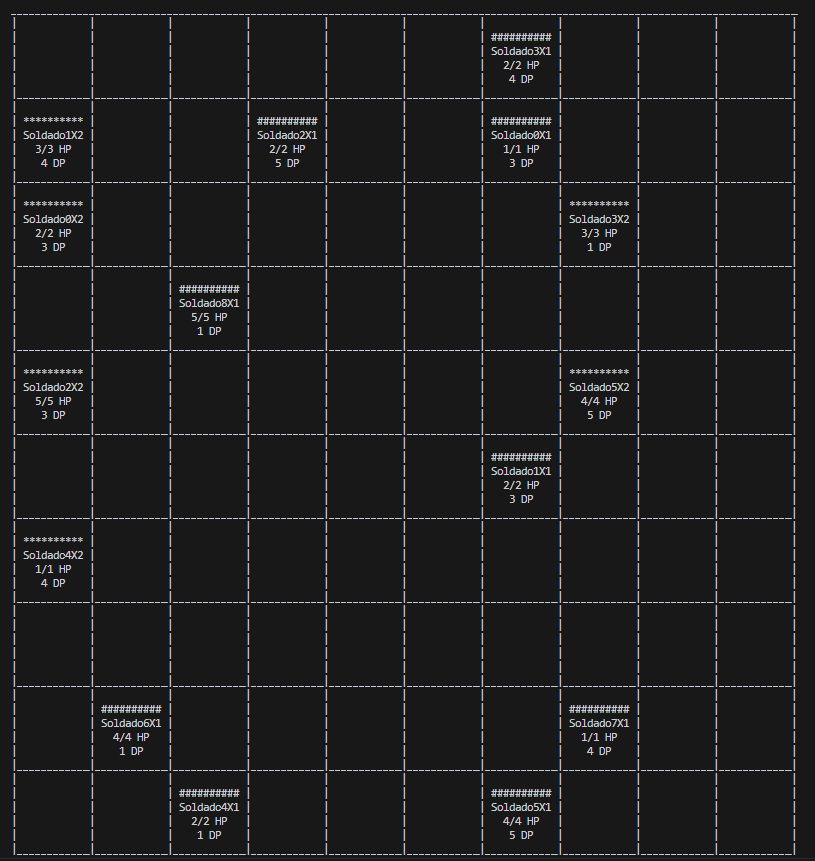
\includegraphics[width=0.6\textwidth,keepaspectratio]{img/tablero.png}
		%\includesvg{img/automata.svg}
		%\label{img:mot2}
		%\caption{Product backlog.}
	\end{figure}
	\begin{figure}[H]
		\centering
	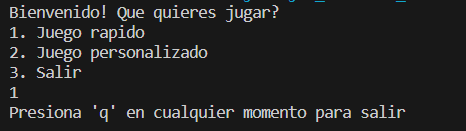
\includegraphics[width=0.6\textwidth,keepaspectratio]{img/menu1.png}
		%\includesvg{img/automata.svg}
		%\label{img:mot2}
		%\caption{Product backlog.}
	\end{figure}
	\begin{figure}[H]
		\centering
	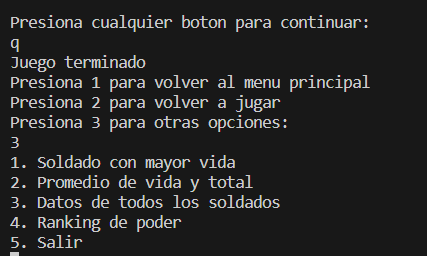
\includegraphics[width=0.6\textwidth,keepaspectratio]{img/menu2.png}
		%\includesvg{img/automata.svg}
		%\label{img:mot2}
		%\caption{Product backlog.}
	\end{figure}
	\begin{figure}[H]
		\centering
	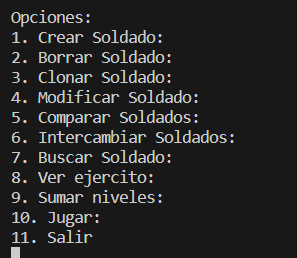
\includegraphics[width=0.6\textwidth,keepaspectratio]{img/menu3.png}
		%\includesvg{img/automata.svg}
		%\label{img:mot2}
		%\caption{Product backlog.}
	\end{figure}
	\begin{figure}[H]
		\centering
	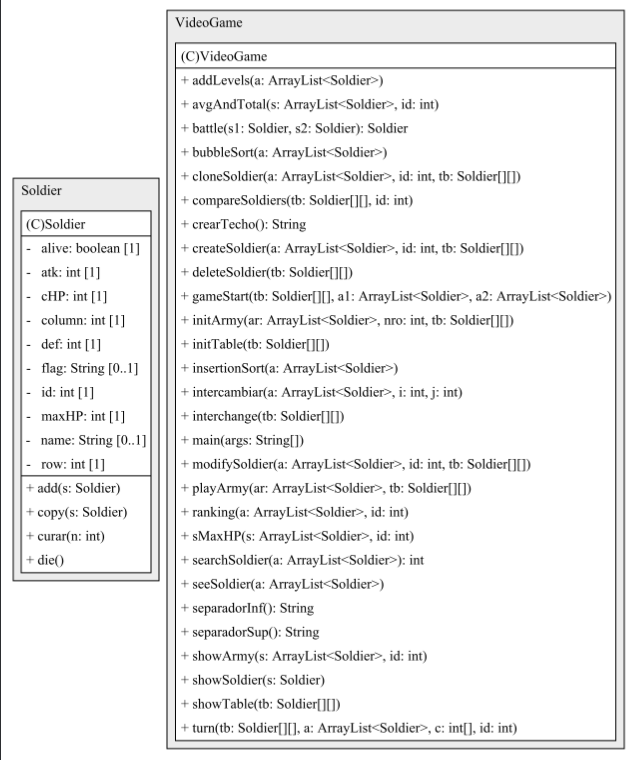
\includegraphics[width=0.6\textwidth,keepaspectratio]{img/uml.png}
		%\includesvg{img/automata.svg}
		%\label{img:mot2}
		%\caption{Product backlog.}
	\end{figure}
	
	
	\section{\textcolor{red}{Rúbricas}}
	
	\subsection{\textcolor{red}{Entregable Informe}}
	\begin{table}[H]
		\caption{Tipo de Informe}
		\setlength{\tabcolsep}{0.5em} % for the horizontal padding
		{\renewcommand{\arraystretch}{1.5}% for the vertical padding
		\begin{tabular}{|p{3cm}|p{12cm}|}
			\hline
			\multicolumn{2}{|c|}{\textbf{\textcolor{red}{Informe}}}  \\
			\hline 
			\textbf{\textcolor{red}{Latex}} & \textcolor{blue}{El informe está en formato PDF desde Latex,  con un formato limpio (buena presentación) y facil de leer.}   \\ 
			\hline 
			
			
		\end{tabular}
	}
	\end{table}
	
	\clearpage
	
	\subsection{\textcolor{red}{Rúbrica para el contenido del Informe y demostración}}
	\begin{itemize}			
		\item El alumno debe marcar o dejar en blanco en celdas de la columna \textbf{Checklist} si cumplio con el ítem correspondiente.
		\item Si un alumno supera la fecha de entrega,  su calificación será sobre la nota mínima aprobada, siempre y cuando cumpla con todos lo items.
		\item El alumno debe autocalificarse en la columna \textbf{Estudiante} de acuerdo a la siguiente tabla:
	
		\begin{table}[ht]
			\caption{Niveles de desempeño}
			\begin{center}
			\begin{tabular}{ccccc}
    			\hline
    			 & \multicolumn{4}{c}{Nivel}\\
    			\cline{1-5}
    			\textbf{Puntos} & Insatisfactorio 25\%& En Proceso 50\% & Satisfactorio 75\% & Sobresaliente 100\%\\
    			\textbf{2.0}&0.5&1.0&1.5&2.0\\
    			\textbf{4.0}&1.0&2.0&3.0&4.0\\
    		\hline
			\end{tabular}
		\end{center}
	\end{table}	
	
	\end{itemize}
	
	\begin{table}[H]
		\caption{Rúbrica para contenido del Informe y demostración}
		\setlength{\tabcolsep}{0.5em} % for the horizontal padding
		{\renewcommand{\arraystretch}{1.5}% for the vertical padding
		%\begin{center}
		\begin{tabular}{|p{2.7cm}|p{7cm}|x{1.3cm}|p{1.2cm}|p{1.5cm}|p{1.1cm}|}
			\hline
    		\multicolumn{2}{|c|}{Contenido y demostración} & Puntos & Checklist & Estudiante & Profesor\\
			\hline
			\textbf{1. GitHub} & Hay enlace URL activo del directorio para el  laboratorio hacia su repositorio GitHub con código fuente terminado y fácil de revisar. &2 &X &2 & \\ 
			\hline
			\textbf{2. Commits} &  Hay capturas de pantalla de los commits más importantes con sus explicaciones detalladas. (El profesor puede preguntar para refrendar calificación). &4 &X &2 & \\ 
			\hline 
			\textbf{3. Código fuente} &  Hay porciones de código fuente importantes con numeración y explicaciones detalladas de sus funciones. &2 &X &2 & \\ 
			\hline 
			\textbf{4. Ejecución} & Se incluyen ejecuciones/pruebas del código fuente  explicadas gradualmente. &2 &X &2 & \\ 
			\hline			
			\textbf{5. Pregunta} & Se responde con completitud a la pregunta formulada en la tarea.  (El profesor puede preguntar para refrendar calificación).  &2 &X &2 & \\ 
			\hline	
			\textbf{6. Fechas} & Las fechas de modificación del código fuente estan dentro de los plazos de fecha de entrega establecidos. &2 &X &2 & \\ 
			\hline 
			\textbf{7. Ortografía} & El documento no muestra errores ortográficos. &2 &X &2 & \\ 
			\hline 
			\textbf{8. Madurez} & El Informe muestra de manera general una evolución de la madurez del código fuente,  explicaciones puntuales pero precisas y un acabado impecable.   (El profesor puede preguntar para refrendar calificación).  &4 &X &4 & \\ 
			\hline
			\multicolumn{2}{|c|}{\textbf{Total}} &20 & &18 & \\ 
			\hline
		\end{tabular}
		%\end{center}
		%\label{tab:multicol}
		}
	\end{table}
	
\clearpage

\section{Referencias}
	\begin{itemize}
		\item Fundamentos de la programación 2 - Tópicos de la programación Orientada a Objetos (Marco Aedo)
	\end{itemize}
	
%\clearpage
%\bibliographystyle{apalike}
%\bibliographystyle{IEEEtranN}
%\bibliography{bibliography}
			
\end{document}
